\section{Preprocessing}

\subsection{What can be preprocessed now?}
Since we have to deal with classification problems, before preprocessing data we must be sure not to apply supervised filters on the whole dataset. If we need supervised filters, we must split the dataset in training set and test set before applying them. However, in our case there is no need for a supervised filters but  attribute selection, so we performed all the unsupervised preprocessing operations at the beginning, postponing the attribute selection after the training/test split.

\subsection{Data Cleaning and Reduction}
Since the Weka framework was not able to parse correctly the source file, for the following operations we used \textit{Microsoft Excel} and \textit{Apple Numbers}.

\subsubsection{Removing Noisy and Irrelevant attributes}
The first preprocessing operation is the attribute reduction, indeed we decided to remove all the features that are not domain-specific, nor useful for classification purposes. Among them we deleted:

\begin{itemize}
	\item \textbf{ID}s: \textit{Bnb\_ID, scrape\_id, host\_id}
	\item \textbf{URL}s: \textit{listing\_url, picture\_url, host\_url, host\_thumbnail\_url, host\_picture\_url}
	\item Scraping informations like \textit{last\_scraped\_date, calendar\_last\_scraped}
	\item Useless information on the rent for classification purposes like \textit{name, description, first\_review\_date}
	\item Useless information about the host like \textit{host\_name, host\_location} (it is not the place in which the rent is, but where the host lives), \textit{host\_about, host\_has\_profile\_pic}
\end{itemize}

\subsubsection{Removing Redundant Attributes}
The next step was the reduction of attributes explicitly redundant. For all of these we did not compute the $\chi^2$ test because of the explicit correlation between the features

\begin{itemize}
	\item \textit{host\_neighbourhood and neighbourhood} \textbf{w.r.t.} the couple \textit{neighbourhood\_cleansed, neighbourhood\_group\_cleansed}
	\item \textit{host\_total\_listings\_count} completely equal to \textit{host\_listing\_count}
	\item \textit{host verification} \textbf{w.r.t.} \textit{host\_identity\_verified}
	\item \textit{minimum\_minimum\_nights, minimum\_maximum\_nights, maximum\_minimum\_night, maximum\_maximum\_nights, minimum\_nights\_avg} and \textit{maximum\_nights\_avg} are redundancies of the \textit{attributes minimum\_nights} and \textit{maximum\_nights}
	\item \textit{review\_scores\_accuracy, review\_scores\_cleanliness, review\_scores\_checkin, review\_scores\_communications, review\_scores\_location, review\_scores\_value} are rounded values that have been more precisely combined in another already-existing attribute that is \textit{review\_scores\_rating}
	\item \textit{calculated\_host\_listings\_count} (+ category) are redundant attributes of \textit{listings\_count} valid only for their respective category
\end{itemize}

\subsubsection{Additional Removed Features}
Eventually, the other columns that have been discarded are:

\begin{enumerate}
	\item Attributes that strongly depend from the instant in which the scraping has been performed like \textit{has\_availability\_now, availability\_30, availability\_60, availability\_90, number\_of\_reviews\_ltm, number\_of\_reviews\_l30}
	\item Empty attributes like \textit{license}, \textit{bathrooms}
	\item Others, like \textit{latitude} and \textit{longitude} that are not more useful than the easier data on the neighborhood
\end{enumerate}


\subsection{Dealing with Missing Fields}



\subsection{Data Transformation}

\subsubsection{Attribute Formats Transformation}
Some of the attributes persisted after the cleaning and reduction phases of the precedent sections were in a not suitable for the knowledge discovery operation that will be done in chapter 3. Thus, we decide to transform those attribute to make them adequate for classification. The features we transformed are: \textit{amenities} (we will discuss them in chapter 2.4.2), \textit{bathrooms}, and \textit{price}.

The \textit{bathrooms} in the scraped file were two columns, one empty and removed and the other one containing string values as "Shared bath", "1 shared bath", "1.5 bath". We manage to format it in two columns, one referring to the number of bathrooms inside the building and the other telling if the bathrooms are shared or not.
\begin{figure}[H]
	\centering
	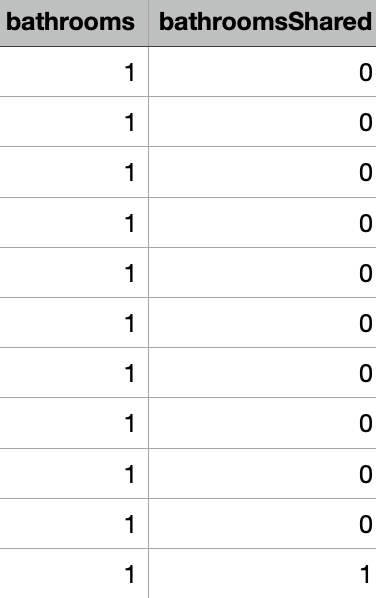
\includegraphics[width=0.3\textwidth]{img/bath.png}  
\end{figure}

The \textit{price} attribute in the original file was a string made of \textit{\$} plus the amount (e.g., \textit{\$170}). We transformed it simply by removing the dollar sign.

\subsubsection{One Hot for the Amenities}
\textit{Amenities}, in the original file, were list of string inputed by the used that contain all the facility the specific BnB offers to the guests.
\begin{figure}[H]
	\centering
	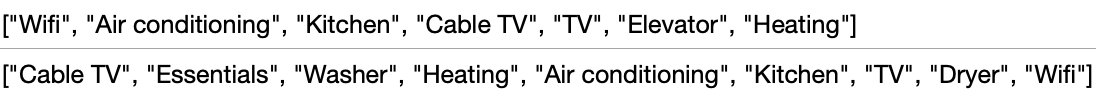
\includegraphics[width=\textwidth]{img/amenities.png}  
\end{figure}

Structured in this way they were difficult to process. Because many machine learning models need their input variables to be numeric, we need to transform these categorical variables using the \textit{one-hot encoding}. One-hot encoding is a frequently used method to deal with categorical data, since many machine learning models need their input variables to be numeric, categorical variables need to be transformed in the pre-processing part.

\textit{"How did we proceed to create the one-hot table?"} First, we collect all the distinct values from the entries in the csv amenitites' column and we created new columns using them, through a first scan of the column. Then we made a second scan to compute the values of each of the newly created attribute: if the attribute name is the same of one is contained in the amenities' list we are considering, then we put a value equal to 1, otherwise we put 0. Obtaining something like this:

\begin{figure}[H]
	\centering
	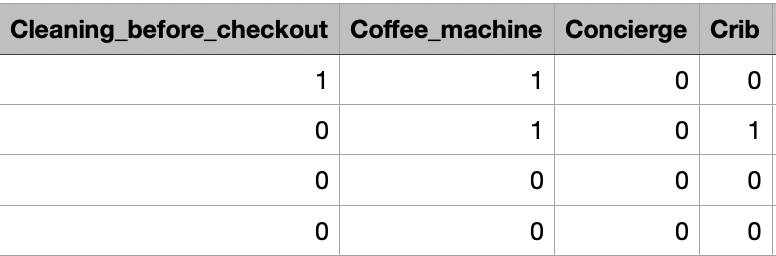
\includegraphics[width=0.6\textwidth]{img/onehot.png}  
\end{figure}

\subsubsection{Amenities' Hot Vector refinements}
The number of columns obtained was very huge, more than three hundreds, so we needed to reduced them in some ways. We notice that few of them were irrelevant and the most of them were redundant, for all of these we did not compute the $\chi^2$ test because of the explicit correlation between the features (\textit{e.g.}, Keurig coffee machine, Coffee maker, Nespresso machine) but we simply merge them.

The irrelevant columns we removed through code, they were: 
\begin{itemize}
	\item \textit{Limited housekeeping u2014 on request}: put just by one user and outdated nowadays;
	\item \textit{Safe}: put just by one user and without a consistent meaning. Without knowing if safe stands that the building is safe or that the BnB is located in a safe location, we decide to remove it.
\end{itemize}

The columns that were similar to each other were merged forming a new columns made of the values of the grouped columns. Merging was done through code, summing they values in each position:

$
	\ \ \ \	\ \ \ \	\ \ \ \	\ \ \ \		new\_column = \sum^{similar \ columns}_{i} columns_i
$

In the case of values inside the \textit{new\_column} greater than 1, we convert back to 1.
The merged columns were (\textit{new name for the column} \textrightarrow \textit{columns merged}):
\begin{itemize}
	\item \textbf{Toiletries} \textrightarrow \textit{1802 Beekman toiletries, Diptyque toiletries, Gilchrist \& Soames toiletries, Malin+Goetz toiletries, Natura toiletries, Toiletries, Neil George toiletries, C.O. Bigelow toiletries,  comfort zone  toiletries, Appelles toiletries, Cote Bastide Argan toiletries, Bio Beauty toiletries, Le Labo toiletries, Elemis toiletries, MOR toiletries}
	\item \textbf{Stove} \textrightarrow \textit{Stainless steel gas stove, Wolf stainless steel gas stove, Viking stainless steel gas stove, Frigidaire stainless steel gas stove, Ge stove, We provide a portable gas stove in our kitchenette.  gas stove, GAS COOK TOP ONLY NO OVEN gas stove, GE stove, Fridgedare 30 inches stainless steel gas stove, Magic Chef  gas stove, Samsung stainless steel gas stove, Stove, Electric stove, LG Stove stainless steel electric stove, Fridgedare stainless steel gas stove, Stainless steel electric stove, Stainless steel stove, Gas stove, Single burner countertop range electric stove, Induction stove, 2 burner hot plate electric stove, Small portable induction stove  electric stove, Two Burner Electric Cook-Top electric stove, GE  electric stove, Stovetop works - Oven does not gas stove}
	\item \textbf{Refrigerator} \textrightarrow \textit{Magic Chef refrigerator, LG refrigerator, Samsung refrigerator, small  refrigerator, Stainless Steel Fridgedare refrigerator, Undercounter refrigerator, bloomberg refrigerator, Gaggenau refrigerator, Kenmore refrigerator, Undercounter Refrigerator refrigerator, Bosch refrigerator, Subzero refrigerator, Beko refrigerator, Whirlpool refrigerator, Americana refrigerator, Magic Chef  refrigerator, Refrigerator, Fridgedare Stainless Steel refrigerator, Sub Zero refrigerator, LG smart Tech refrigerator, Inc refrigerator, Frigidaire refrigerator, GE refrigerator, Ge refrigerator}
	\item \textbf{Sound system} \textrightarrow \textit{Built-in sound system in the apartment. sound system, Tivoli Audio Bluetooth sound system, Bluetooth sound system, Unknown - you can plug right into phone sound system with aux, Sonos over WiFi with built-in speakers throughout the house and backyard sound system, BOSE sound system with Bluetooth and aux, Marshall  sound system with Bluetooth and aux, Marshall  Bluetooth sound system, Bose Surround Speaker System in All Rooms sound system with Bluetooth and aux, Roku Bluetooth sound system, roku tv Bluetooth sound system, Echo Dot Bluetooth sound system, bose speaker Bluetooth sound system, Sound system, Bose sound system, Sound system with Bluetooth and aux, Yamaha Bluetooth sound system, Sonos sound system, Sonos Bluetooth sound system, Marshall sound system with Bluetooth and aux, Harman Kardon Bluetooth sound system, Cambridge Audio Bluetooth sound system, Sound system with aux, Samsung Bluetooth sound system, Bose sound system with Bluetooth and aux, Bose Bluetooth sound system, Yamaha sound system with Bluetooth and aux}
	\item \textbf{Linens} \textrightarrow \textit{Supmia linens, Sferra  linens, Bed linens, Frette linens, Sferra linens,  linens}
	\item \textbf{Breakfast} \textrightarrow \textit{Cooked-to-order breakfast available u2014 \$30 per person per day, Breakfast buffet available u2014 \$25 per person per day, Complimentary breakfast, Cooked-to-order breakfast available u2014 \$25 per person per day, Complimentary continental breakfast, Hot breakfast available u2014 \$20 per person per day, Complimentary hot breakfast, Cooked-to-order breakfast available for a fee, Breakfast, Cooked-to-order breakfast available u2014 \$15 per person per day, Continental breakfast available u2014 \$29 per person per day}
	\item \textbf{Air conditioning} \textrightarrow \textit{ICE Air conditioner, Central air conditioning, Air conditioning, Portable air conditioning}
	\item \textbf{Dryer} \textrightarrow \textit{Dryer, Hair dryer, Dryer u2013u00a0In unit, Dryer u2013 In building}
	\item \textbf{Extra pillows} \textrightarrow \textit{Extra pillows and blankets, Bed sheets and pillows}
	\item \textbf{Parking} \textrightarrow \textit{Free street parking, Paid parking lot on premises, Paid parking on premises u2013 1 space, Self-parking u2014 \$35/day, Valet parking u2014 \$65/day, Valet parking u2014 \$75/day, Paid street parking off premises, Valet parking u2014 \$80/day, Paid parking garage on premises u2013 1 space, Valet parking u2014 \$45/day, Paid parking on premises, Paid parking off premises, Self-parking u2014 \$19/day, Free driveway parking on premises, Paid parking lot on premises u2013 1 space, Free driveway parking on premises u2013 1 space, Self-parking u2014 \$40/stay, Valet parking u2014 \$85/day, Paid parking garage on premises, Valet parking u2014 \$70/day, Free parking on premises, Paid valet parking on premises, Self-parking u2014 \$50/day, Paid parking lot off premises, Paid parking garage off premises, Valet parking u2014 \$40/day}
	\item \textbf{Wifi} \textrightarrow \textit{Wifi u2013 500 Mbps, Pocket wifi, Wifi u2013 60 Mbps, Wifi u2013 200 Mbps, Wifi u2013 100 Mbps, Wifi u2013 24 Mbps, Free wifi, Wifi u2013 870 Mbps, Wifi, Wifi u2013 400 Mbps}
	\item \textbf{Oven} \textrightarrow \textit{Frigedare stainless steel oven, Frigidaire stainless steel oven, Oven, GE oven, Stainless steel oven, Toaster oven oven, Samsung stainless steel oven, Fridgedare oven, Power Airfryer 360 stainless steel oven, Small portable oven oven, Wolf stainless steel oven, Frigidaire oven, Viking stainless steel oven, electric  stainless steel oven, large toaster oven oven}
	\item \textbf{Garden} \textrightarrow \textit{Onsite bar u2014 Clinton Hall \& Rooftop Beer Garden, Garden, Onsite restaurant u2014 Clinton Hall \& Rooftop Beer Garden, Garden or backyard}
	\item \textbf{Heating} \textrightarrow \textit{Heating, Radiant heating, Central heating}
	\item \textbf{Kitchen} \textrightarrow \textit{Kitchenette, Kitchen}
	\item \textbf{Onside bar} \textrightarrow \textit{Onsite bar u2014 Gleason's Tavern, Onsite bar u2014 Crown Shy, Onsite bar u2014 Molyvos Restaurant - Bar, Onsite rooftop bar u2014 Make Believe, Onsite bar u2014 The National, Onsite bar, Minibar, face\&body bar Bergman Kelly body soap, Onsite bar u2014 The Seville, Barbecue utensils
	\item \textbf{Onside restaurant} \textrightarrow \textit{Onsite restaurant u2014 Above SIXTY SoHo, Onsite restaurant u2014 Gleason's Tavern, Onsite restaurant u2014 Butter, Onsite restaurant u2014 Parker \& Quinn, Onsite restaurant u2014 Blue Ribbon Sushi Izakaya, Onsite restaurant u2014 Caf u00e9 Hugo, Onsite restaurant u2014 Scarpetta, Onsite restaurant u2014 Park Cafe, Restaurant, Onsite restaurant u2014 Caf u00e9 Boulud, Onsite restaurant u2014 Broome Caf u00e9, Onsite restaurant u2014 The National, Onsite restaurant u2014 Blue Park Kitchen}
	\item \textbf{Pool} \textrightarrow \textit{Pool, Outdoor pool}
	\item \textbf{Washer} \textrightarrow \textit{Washer u2013 u00a0In building, Washer, Dishwasher, Washer u2013 u00a0In unit}
	\item \textbf{Hot water} \textrightarrow \textit{Hot water, Hot tub}
	\item \textbf{Gym} \textrightarrow \textit{24-hour fitness center, Gym, Fitness center}
	\item \textbf{Coffee machine} \textrightarrow \textit{Keurig coffee machine, Coffee maker, Nespresso machine, Pour Over Coffee}
	\item \textbf{Clothing storage} \textrightarrow \textit{Clothing storage, Clothing storage-closed}
}
\end{itemize}




